\documentclass[a4paper,11pt]{article}
\usepackage{amssymb}
\usepackage{mathbbold}
\usepackage{latexsym}
\usepackage{amsmath}
\usepackage{url}
\usepackage{graphicx}
\usepackage{amsthm}
\parindent=0in
\author{Bi Ran(U087272L)}
\title{Hand Written Digit Recognition and Its Improvement}
\frenchspacing

\begin{document}
\maketitle
\begin{abstract}
Handwritten digits recognition is a classic problem of machine learning. The objective is to recognize images of single handwritten digits(0-9). This paper will apply C4.5 decision tree, pairwise C4.5, boosted C4.5, and support vector machine(SVM) on this problem, compare their performance, and finally propose a method to improvement the classification accuracy by adding attributes into data set.
\end{abstract}
\section{Introduction}
Handwritten digit recognition recognition is a classification problem. The performance of classification algorithm heavily depends on properties of data set.
In this paper, Semeion Handwritten Digit Data Set is used for training and testing. The first part of the paper will show the testing result of C4.5, boosted C4.5 and SVM algorithms. We also introduce a optimized version of C4.5 algorithm: pairwise C4.5, which outperforms C4.5 on Semeion data set. Parameter search is applied to achieve relatively good performance for C4.5 and SVM.
The second part will introduce a method to improve accuracy of classifiers by adding extra features into data set. It will be shown that performances of all three algorithms have significant improvement on the modified data set, and SVM with RBF kernel achieves error rate of 3.2643\%.
\section{Background and Motivation}
Handwritten digit recognition has important usage such as recognizing zip code, online recognition on computer tablets. Algorithms like support vector machine and multi layer perceptron are commonly used on this problem, and impressive result has been achieved. Lenet and its boosted version managed to get error rate less than 1\% on MNIST data set\cite{Kussul_improvedmethod}. Decision tree is rarely applied on this problem, SVM gives one of the algorithms which gives the lowest error rate on this problem. It is interesting to see whether it is possible to achieve high accuracy from decision tree algorithm, and improve the performance of SVM. These two completely different algorithm are also used to support the method mentioned in the second part of the paper.
\section{Data set}
Semeion Handwritten Digit Data Set(\url{http://archive.ics.uci.edu/ml/datasets/Semeion+Handwritten+Digit}) is used in this paper. 1593 handwritten digits from around 80 persons were scanned, stretched in a rectangular box 16x16 in a gray scale of 256 values.Then each pixel of each image was scaled into a boolean (1/0) value using a fixed threshold. This data set contains no missing values.\\
Each person wrote on a paper all the digits from 0 to 9, twice. The commitment was to write the digit the first time in the normal way (Figure 1) and the second time in a fast way (Figure 2).
\begin{figure}
\centering
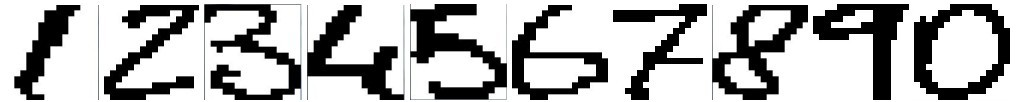
\includegraphics[width=1.0\textwidth]{clear}
\caption{written in normal way}
\end{figure}

\begin{figure}
\centering
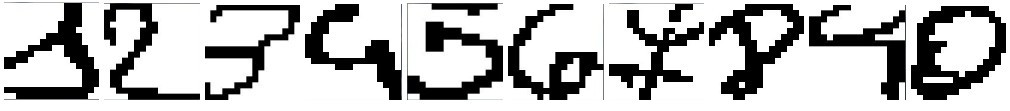
\includegraphics[width=1.0\textwidth]{unclear}
\caption{written in fast way}
\end{figure}
This data set consists of 1593 instances and 256 features for each instance. Each instance represents a handwritten digit, originally scanned with a resolution of 256 grays scale.
Each pixel of the each original scanned image was first stretched, and after scaled between 0 and 1 (setting to 0 every pixel whose value was under the value 127 of the grey scale (127 included) and setting to 1 each pixel whose original value in the grey scale was over 127).
Finally, each binary image was scaled again into a 16x16 square box (the final 256 binary attributes).
The order of the examples in the data set is shuffled before training and testing, because the label distribution of the original data set is not random.
\section{Evaluation}

In this paper, cross validation is used to perform testing. \\
By applying cross validation on different fold number using C4.5 algorithm, we observe that the error rate almost keeps still after 8 fold. 8-folds cross validation is very likely to provide accurate estimation of the real error rate on unseen data. In this paper, we apply 10-folds cross validation on the whole Semeion Handwritten Digit Data Set, and compare the error rates of different algorithms.\\
\emph{WEKA}(\url{http://www.cs.waikato.ac.nz/ml/weka/}) is used for training and testing of C4.5 and boosted C4.5 algorithm. \emph{libsvm} package\cite{LIBSVM} is used for training and testing SVM in this paper.\\
\vspace{0.5cm}\\
\begin{tabular}{c c}
Fold Number & Error Rate\\
\hline \hline
2  &29.0019\%\\
4  &25.6121\%\\
6  &24.231 \%\\
8  & 24.6704\%\\
10 & 23.9799\%\\
12 & 24.8588\%\\
14 & 24.5449\%\\
\end{tabular}
\vspace{0.5cm}\\
\section{Testing}
\subsection{C4.5}
Decision tree is a popular algorithm in data mining and machine learning. There are many decision tree algorithms. We only apply C4.5 in this paper. C4.5 is an improved version of ID3 decision tree. It follows a simple inductive bias, which is ``smaller trees are preferred''. This inductive bias is motivated by Occan's Razor principle, and it works well in practice.\\
To further simplify the decision tree to avoid over fitting problem, C4.5 perform pruning to limit the size of the tree. To achieve good performance, we perform parameter search on two parameters: $C$ and $minObj$. \\
$C$ is confident factor, which is a probability threshold of the probability of the actual error rate being worse than the pessimistic estimation\cite{Morgan.Kaufmann}. The pessimistic estimation of the error rate for each subtree is used when do the subtree replacement and subtree raising pruning in C4.5 algorithm. Smaller confidence factor implies more pessimistic estimation, which will cause more drastic pruning.\\
The $minObj$ variable limit the minimum number of examples each leaf can have. This constrain can help reduce the size of the tree, thus makes the tree more robust to the effect of noise.
\vspace{0.5cm}\\
\begin{tabular}{c|c c c c}
C$\backslash$ minObj	&1		&2		&3		&4\\
\hline \hline
1e-3 	&24.6077 \%	&24.3566 \%	&24.1682 \%	 &24.6704 \%\\
1e-2	&24.4193 \%	 &24.4821 \%	&24.231  \%	 &24.5449 \%\\
1e-1	&24.6077 \%	&24.231  \%	&24.231  \%	 &24.6077 \%\\
0.5 &24.2938 \%     &24.0427 \% &24.1055 \%  &24.8588 \%\\
1	&24.6077 \%	    &23.7916 \%	&24.1682 \%	 &24.796  \%\\
\end{tabular}
\vspace{0.5cm}\\
The result in the table above shows that he error rate of C4.5 algorithm is lowest when $C=1$ and $minObj=2$, which gives error rate of 23.7916\%. The differences between error rates are very small, which implies that pruning does not help much in this data set.\\
This result is very poor compared to many other popular algorithms like support vector machine(will see it later). There are some possible reasons:\\
\begin{enumerate}
\item[1] Decision tree algorithm itself has limitation. The problem of learning optimal decision tree is NP-complete\cite{DT_NPC}. C4.5 use a greedy algorithm, which does not guarantee to find the optimal decision tree.
\item[2] Although decision tree can estimate any discrete functions, it is difficult to learn certain functions. e.g. OXR function is hard to learn by decision tree, because the minimal decision tree for XOR requires a full binary tree , and it is hard to find ``small'' trees to estimate XOR.
\item[3] Although C4.5 decision tree supports multi-class classification problem, more classes would result in larger trees. For example, if there are $N$ classes, and each attribute is binary. Since each leaf can only represent one class, the height of the tree must be larger than $log_2(N)$. If the size of decision trees generated by C4.5 follows some fixed distribution, then the size of decision tree tends to become larger when the minimal possible tree size becomes larger. Larger tree would contradict to Occan's Razor principle. Thus, C4.5 may not perform well in multi-class classification problems.
\end{enumerate}
\subsection{Pairwise C4.5}
The first two reasons above are limitations of decision tree, which is hard to overcome. The 3rd one can be overcame by converting multi-class classification problem into two-class classification problem.\\
Several possible methods can be used for this conversion. We only consider ``pairwise'' method in this paper. Pairwise method train $N*(N-1)/2$ classifiers for each pair of classes($N$ is the number of classes). When classifying a new instance, each classifier vote for the class based on their classification results. The class with the highest vote is considered as the classification result. If draw happens, randomly choose one of the classes with the highest vote.\\
Weka itself does not support this conversion. I wrote a separate program based on WEKA's library to perform this test\footnote{Source code is available at \url{http://code.google.com/p/cs2306-machine-learning/source/browse/#svn/trunk/src}}.\\
\vspace{0.5cm}\\
\begin{tabular}{c c}
Algorithm	& Error rate\\
\hline \hline
original C4.5	& 23.7916\%\\
pairwise C4.5	& 15.5345\%\\
\end{tabular}
\vspace{0.5cm}\\
We can see from the table that pairwise C4.5 performs much better than original C4.5. This is because in pairwise C4.5, although there are more decision trees, the size of each tree is small(about 20 on average). However, the size of the tree for the original C4.5 is 293. Thus, pairwise C4.5 performs better, since small trees are more likely to generalize well on unseen data.
\subsection{Boosting}
Boosting is an algorithm which aims to boost weak classifier into a strong classifier. The boosting algorithm used in this paper is AdaBoosting M1 provided in WEKA.\\
The boosting algorithm constructs the classifier by several iterations, each iteration obtains a classifier by a weighted data set, and the output of the final classifier is obtained by weighted sum of the results of all classifiers. After each iteration, data set is reweighted, and misclassified instances has a larger weight so that they are paid more attention to in the next iteration. The weight of each classifier is decided by their accuracy. Boosting works well with decision tree in practice, and it often does not suffer from over fitting problem.\\
Following result is obtained by applying boosting on C4.5 algorithm with different number of iterations.\\
\vspace{0.5cm}\\
\begin{tabular}{c c}
\# of Iterations	& Error rate\\
\hline \hline
	2		& 23.7916\%\\
	4		& 17.7024\%\\
	8		& 13.4965\%\\
	16		& 9.6673\%\\
    32      & 7.7841\%\\
    64      & 6.6541\%\\
\end{tabular}
\vspace{0.5cm}\\
From the table, we can see that the error rate drops rapidly when the number of iteration grows. Although higher accuracy can be achieved by further increase the number of iterations, the error rate would stop decreasing or start to increase(over fitting) at last.\\
Boosting algorithm constructs a classifier by combining several classifiers, which intuitively increase the complexity of the classifier. However, according to Occan's Razor principle, simpler classifiers tend to generalize better on unseen data. Boosting algorithm seems a contradict with Occan's Razor principle.\\
One possible explanation is that the complexity of classifier is not measured by the number of classifiers, but by the ``margin'' of the classifier.
In Boosting algorithm, each classifier vote for a class with its weight, and the class with the highest weight is the result of classification. The margin of an example is defined by the difference between weight of correct class, and the sum of all weights of incorrect class. The larger the margin is, the more confident the classification for this instance is. The boosting algorithm tend to maximize margin of instances, and convergence with some large margin distribution\cite{boosting}.\\
\subsection{Boosted Pairwise C4.5}
We can also apply boosting on Pairwise C4.5. The result is shown in the table below\footnote{Source code is available at \url{http://code.google.com/p/cs2306-machine-learning/source/browse/#svn/trunk/src}}:\\
\vspace{0.5cm}\\
\begin{tabular}{c c c}
\# of Iterations	& Boosted C4.5 & Boosted Pairwise C4.5\\
\hline \hline
	2		& 23.7916\% & 15.283\%  \\
	4		& 17.7024\% & 12.075\%  \\
	8		& 13.4965\% & 9.3710\%  \\
	16		& 9.6673\%  & 8.0503\%  \\
    32      & 7.7841\%  & 6.8553\%\\
\end{tabular}
\vspace{0.5cm}\\
The result shows that boosted Pairwise C4.5 algorithm over performs boosted C4.5 algorithm, which is not surprising.\\

\subsection{Support Vector Machine}
Support vector machine can be seen as a generalized version of linear classifier. SVM maps each instance into a higher dimensional feature space, and look for a hyper plane, which separate different classes. Hyper plane with large margin is preferred. All calculation of feature vector with high dimension can be done via kernel function, which makes training and testing terminates in feasible time. Although new kernel functions are being purposed by researchers, four basic kernels are the most popular\cite{SVM}:
\begin{itemize}
\item linear: $K(x_i,x_j)=x_i^Tx_j$\\
\item polynomial: $K(x_i,x_j)=(\gamma x_i^Tx_j+r)^d$, $\gamma >0$\\
\item radial basis function (RBF): $K(x_i,x_j)=\exp(-\gamma + \|x_i-x_j\|^2)$, $\gamma > 0$\\
\item sigmoid: $K(x_i,x_j)=tanh(\gamma x_i^Tx_j+r)$\\
\end{itemize}
According to \cite{SSK} and \cite{LL}, linear kernel is a special case of RBF kernel, and sigmoid kernel behaves like RBF kernel with certain parameters. Thus in this paper, we only use RBF kernels.\\
There are many kinds of SVMs based on different error function. In this paper, we simply use C-svm, which minimize error function:
    $$\frac{1}{2}\|\vec{\beta}\|^2+C\sum_{i=1}^n \xi_i$$
 subject to:$$y_i(\vec{\beta}\cdot \vec{x_i}+\beta{0})\geq 1-\xi_i$$$$\forall i, \xi_i\geq 0$$

Note that $C$ in the error function, and $\gamma$ in the kernel function are adjustable parameters. To find the optimal parameter, we can use grid-search\cite{SVM}: construct exponential growth sequence of $C$ and $\gamma$, and use a coarse grid search and cross validation to find a ``better'' region. Apply more accurate grid search on that region to find the best parameters. Grid search is a greedy algorithm, which gives local optimal result. In this paper, tools provided in libsvm\cite{LIBSVM} package are used to perform the model selection automatically.\\
As shown in Figure 3, the SVM tends to have better performance when $C=2.0$ and $\gamma=0.0078125$, and the error rate achieved is 4.2059\%.

\begin{figure}
\centering
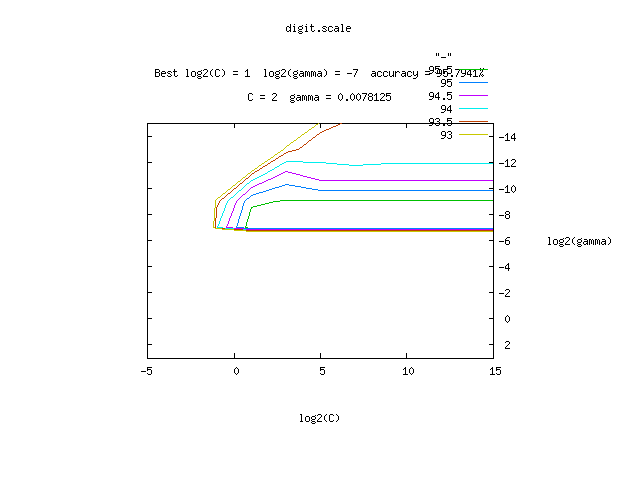
\includegraphics[width=1.0\textwidth]{digit}
\caption{grid search on $C,\gamma$}
\end{figure}

\section{Improvement}
\subsection{Motivation}
One observation from the algorithms is that neither decision tree nor SVM makes use of the information about the order of attributes. Actually, if some fixed permutation is applied on the attributes of each example in the data set, then decision tree and SVM will generate the same model as the model generated by original data set(subtle difference may exists, which depends on how the algorithm deals with ``tie conditions'', e.g. two attributes have the same information gain in C4.5).\\
However, the positions of pixel are important for human when recognizing a image. If the pixel of an image randomly rearranged, it is very difficult, or impossible to recognize the image for human. If decision tree and SVM can make use of these information, their performance can be expected to have further improvement.\\

\subsection{Adding Features}
One possible solution is to make position information of pixels available to algorithms. In this paper, we try to add some attributes derived by position information.\\
We choose to add $16$ extra features $r[16]$, one for each row, which describes how many ``black segments'' are there in the row. For example, in a image of ``1'', most of $r[i]$ can be expected to be $1$; in a image of ``0'', most $r[i]$ can be expected to be 2, and a few can be 1. Similarly, 16 more features $c[16]$ are added for each column, which means the number of ``black segments'' in each column.\\
The variance of the number of black pixels in each row and column are also added into each example, which can bring in some information about the distribution of pixels.\\
34 extra features are added into each examples in total. Thus the modified data set has 290 features for each example.
\subsection{Testing On Modified Data Set}
\vspace{0.5cm}
\begin{tabular}{c c c}
Algorithm		&	Original Data	&Modified Data\\
\hline \hline
C4.5                            &23.7916\%		& 18.5813\%\\
Pairwise C4.5                   &15.5345\%      & 12.3899\%\\
Boosted C4.5(32 iter)	        &7.7841\%		& 4.5198\%\\
Boosted PW C4.5(32 iter)	    &6.8553\%       & 5.2830\%\\
SVM                         	&4.2059\%       & 3.2643\%\\
\end{tabular}
\vspace{0.5cm}\\
From the result, we can see that all algorithms' error rates on modified data drop to some extent.\\
\subsection{Analysis}
By ranking the information gain of all attributes of the data set, in top 15 features, 14 of them are newly added features; 21 out of top 34 new features ranks less than 30. \\
In the decision tree constructed for the new data set, new features are made heavily used of. The size of the new tree is 229, which is smaller than the size of the tree for the old data set, which is 293. According to the inductive bias of C4.5, smaller trees tends to generalize better. So C4.5 can perform better on the modified data set.\\
SMO algorithm gives 139 support vectors when trained by the whole original data set, while only 115 is obtained on the new data set. The number of support vectors can be seen as a measure of complexity of the classifier. SVM have better performance on the new data set can be considered as the result of Ocam's Razor principle.\\
Although adding extra features makes data set more complicated, it actually makes classifiers simpler, thus generalize better.
\subsection{Testing on MNIST Data set}
MNIST(\url{http://yann.lecun.com/exdb/mnist/}) is a popular handwritten digit data set. This data set contains 60000 instances for training, and 10000 instances for testing. To make time cost feasible, we make a random sample of 1800 instances from the training set for training purpose. We use the whole testing data set(10000 instance) for testing, because testing is relatively fast, and large testing set would give closer result to the real accuracy on unseen data. The range of feature in the original data set is 0 to 256, which is too large. We normalize attributes of instances to range from 0 to 1. This is to avoid attributes in greater numeric ranges dominate those in smaller numeric ranges. Another advantage is to avoid numerical difficulties when calculating vector inner product\cite{SVM}.We do not need to normalize the Semeion data set because the range of features are between 0 and 1 initially. Grid search showed that $C=8, \gamma=0.0078125$ gives relatively good performance.\\
\vspace{0.5cm}
\begin{tabular}{c c}
Data Set	& Error rate\\
\hline \hline
MNIST	                  & 6.4\%\\
MNIST(extra features)	  & 5.72\%\\
\end{tabular}
\vspace{0.5cm}\\
The error rate reduces as expected when adding extra features. \\
This technique can be expected to work on general image classification problem whose data set only contains information about pixels color of images.

\section{Further Work}
\begin{itemize}
 \item How Pairwise C4.5 performs on other multi-class classification problems.
 \item Apply other method to build multi-class C4.5 based on 0-1 C4.5(e.g. one-versus-all).
 \item Whether adding more features derived from position information of pixels could further improve the accuracy, and whether improvement may be observed on other algorithms.
\end{itemize}
\section{Conclusion}
Comparing performance of different algorithms on on Semeion Data Set, C4.5 algorithm performs poorly, and adjusting parameters doesn't change the result much; Pairwise C4.5 performs better than C4.5 on this data set. Boosted C4.5 has a much better performance, and similar for Boosted Pairwise C4.5. C-SVM with RBF kernel manages to reach 4.2059\% error rate after parameter search. Adding extra features into the data set, the error rate for all these algorithm drops to some extent, and SVM achieves error rate of 3.2643\%. Improvement of SVM is also observed on MNIST data set by adding extra features, and this technique can be expected to generalize on other image classification problems.

\newpage
\bibliographystyle{h-physrev3}
\bibliography{ref}
\end{document}
